
\documentclass{article}

\usepackage[a4paper,margin=5pt]{geometry}

\usepackage[T1]{fontenc}
\usepackage{times,multicol,graphicx}
\usepackage{xcoffins}

\usepackage{times,color}
\newcommand\cbox[2][.8]{{\setlength\fboxsep{0pt}\colorbox[gray]{#1}{#2}}}

\ExplSyntaxOn

\ExplSyntaxOff



%\scrollmode

\pagestyle{empty}

\begin{document}

  \NewCoffin \result
  \NewCoffin \aaa
  \NewCoffin \bbb
  \NewCoffin \ccc
  \NewCoffin \ddd
  \NewCoffin \eee
  \NewCoffin \fff
  \NewCoffin \rulei
  \NewCoffin \ruleii
  \NewCoffin \ruleiii

\SetHorizontalCoffin \result {}
\SetHorizontalCoffin \aaa {\fontsize{52}{50}\sffamily\bfseries mitteilungen}
\SetHorizontalCoffin \bbb {\fontsize{52}{50}\sffamily\bfseries typographische}
\SetHorizontalCoffin \ccc {\fontsize{12}{10}\sffamily
                      \quad zeitschrift des bildungsverbandes der
                      deutschen buchdrucker leipzig
                     \textbullet{} oktoberheft 1925}
\SetHorizontalCoffin \ddd {\fontsize{28}{20}\sffamily sonderheft}
\SetVerticalCoffin \eee {180pt}
                 {\raggedleft\fontsize{31}{36}\sffamily\bfseries
                      elementare\\
                      typographie}
\SetVerticalCoffin \fff {140pt}
                 {\raggedright \fontsize{13}{14}\sffamily\bfseries
                       natan altman \\
                       otto baumberger \\
                       herbert mayer \\
                       max burchartz \\
                       el lissitzky \\
                       ladislaus moholy-nagy \\
                       moln\'ar f.~farkas \\
                       johannes molzahn \\
                       kurt schwitters \\
                       mart stam \\
                       ivan tschichold}

\RotateCoffin \bbb {90}
\RotateCoffin \ccc {270}

\SetHorizontalCoffin \rulei  {\color{red}\rule{6.5in}{1pc}}
\SetHorizontalCoffin \ruleii {\color{red}\rule{1pc}{23.5cm}}
\SetHorizontalCoffin \ruleiii{\color{black}\rule{10pt}{152pt}}


\JoinCoffins \result                \aaa
\JoinCoffins \result[\aaa-t,\aaa-r] \rulei   [b,r](0pt,2mm)
\JoinCoffins \result[\aaa-b,\aaa-l] \bbb     [B,r](2pt,0pt)
\JoinCoffins \result[\bbb-t,\bbb-r] \ruleii  [t,r](-2mm,0pt)
\JoinCoffins \result[\aaa-B,\aaa-r] \ccc     [B,l](66pt,14pc)
\JoinCoffins \result[\bbb-l,\ccc-B] \fff     [t,r](-2mm,0pt)
\JoinCoffins \result[\fff-b,\fff-r] \ruleiii [b,l](2mm,0pt)
\JoinCoffins \result[\ccc-r,\fff-l] \eee     [B,r]
\JoinCoffins \result[\eee-T,\eee-r] \ddd     [B,r](0pt,4pc)


\vspace*{3cm}
\begin{center}
  {\Large Title page of ``elementare typographie'' by Ivan Tschichold\par}

\large
\vspace*{1cm}

  1. first the scanned original from 1925

\vspace*{6mm}

  2. then the recreated \TeX{} version from 2010 using coffins---not
     attempting\\ to match the fonts and size but the structure

\vspace*{6mm}

  3. and finally the source code used.

     This document uses the new
     implementation by Joseph in \texttt{l3coffins-new}.

\end{center}

\newpage


\begin{center}
  \null
  \fbox{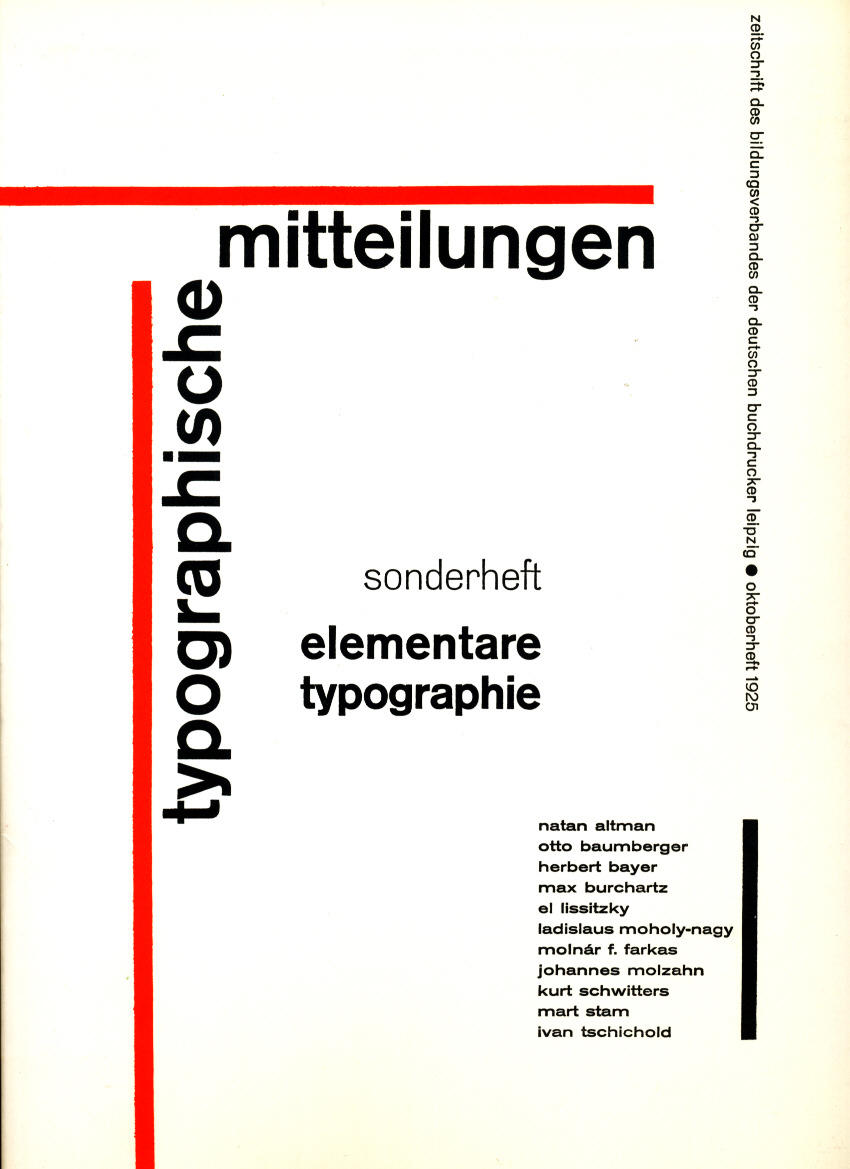
\includegraphics[scale=.95]{elementare-typographie-title.jpg}}
\end{center}

\newpage

\TypesetCoffin \result

\newpage

\vspace*{3cm}
\begin{center}
  {\Large Code used: \par}
\vspace*{1cm}


\begin{minipage}{14cm}
\begin{verbatim}
\SetHorizontalCoffin\result{}
\SetHorizontalCoffin \aaa {\fontsize{52}{50}\sffamily\bfseries mitteilungen}
\SetHorizontalCoffin \bbb {\fontsize{52}{50}\sffamily\bfseries typographische}
\SetHorizontalCoffin \ccc {\fontsize{12}{10}\sffamily
                      \quad zeitschrift des bildungsverbandes der
                      deutschen buchdrucker leipzig
                     \textbullet{} oktoberheft 1925}
\SetHorizontalCoffin \ddd {\fontsize{28}{20}\sffamily sonderheft}
\SetVerticalCoffin \eee {180pt}
                 {\raggedleft\fontsize{31}{36}\sffamily\bfseries
                      elementare\\
                      typographie}
\SetVerticalCoffin \fff {140pt}
                 {\raggedright \fontsize{13}{14}\sffamily\bfseries
                       natan altman \\
                       otto baumberger \\
                       herbert mayer \\
                       max burchartz \\
                       el lissitzky \\
                       ladislaus moholy-nagy \\
                       moln\'ar f.~farkas \\
                       jahannes molzahn \\
                       kurt schwitters \\
                       mart stam \\
                       ivan tschichold}

\RotateCoffin \bbb {90}
\RotateCoffin \ccc {270}

\SetHorizontalCoffin \rulei  {\color{red}\rule{6.5in}{1pc}}
\SetHorizontalCoffin \ruleii {\color{red}\rule{1pc}{23.5cm}}
\SetHorizontalCoffin \ruleiii{\color{black}\rule{10pt}{152pt}}

\JoinCoffins \result                \aaa
\JoinCoffins \result[\aaa-t,\aaa-r] \rulei   [b,r](0pt,2mm)
\JoinCoffins \result[\aaa-b,\aaa-l] \bbb     [B,r](2pt,0pt)
\JoinCoffins \result[\bbb-t,\bbb-r] \ruleii  [t,r](-2mm,0pt)
\JoinCoffins \result[\aaa-B,\aaa-r] \ccc     [B,l](66pt,14pc)
\JoinCoffins \result[\bbb-l,\ccc-B] \fff     [t,r](-2mm,0pt)
\JoinCoffins \result[\fff-b,\fff-r] \ruleiii [b,l](2mm,0pt)
\JoinCoffins \result[\ccc-r,\fff-l] \eee     [B,r]
\JoinCoffins \result[\eee-T,\eee-r] \ddd     [B,r](0pt,4pc)
\SetHorizontalCoffin\result{}
\SetHorizontalCoffin \aaa {\fontsize{52}{50}\sffamily\bfseries
                       mitteilungen}
\SetHorizontalCoffin \bbb {\fontsize{52}{50}\rotatebox{90}{\sffamily\bfseries
                      typographische}}

\TypesetCoffin \result
\end{verbatim}

This is not necessarily the final syntax but for now it does its job. For
example, flexible support for adding ornaments (lines, \ldots) is still
missing, so above the rules got added as predefined individual coffins.

\end{minipage}
\end{center}

\end{document}

